\chapter{Návrh a implementácia riadiaceho systému robota.}
Základom nami použitého riadiaceho systému budú dva PID reglátory zapojené do kaskády. Toto zapojenie budeme ďalej označovať ako \ac{RS}. Vstupom RS bude požiadavka na rýchlosť pohybu robota v $rad.s^{-1}$ a výstupom strieda PWM signálu privádzaná na vstup do H-mostíka, vyjadrená hodnotou od -100\% až 100\% (kde záporná hodnota predstavuje zmenu smeru otáčania motorov). Funkcia jednotlivých PID regulátorov v RS bude vysvetlená v nasledujúcej časti práce. Autor považuje za nutné podotknúť, že samotné zabezpečenie balansovania robota na mieste je možné zabezpčiť použitím jediného PID regulátora. Nevýhodou takéhoto postupu je ale nemožnosť akejkoľvek regulácie rýchlosti pohybu robota. 

\section{Štruktúra RS robota}

Na \figurename~\ref{fig:RS} sme znázornili zapojenie PID regulátorov v RS.  

\begin{figure}
\centering
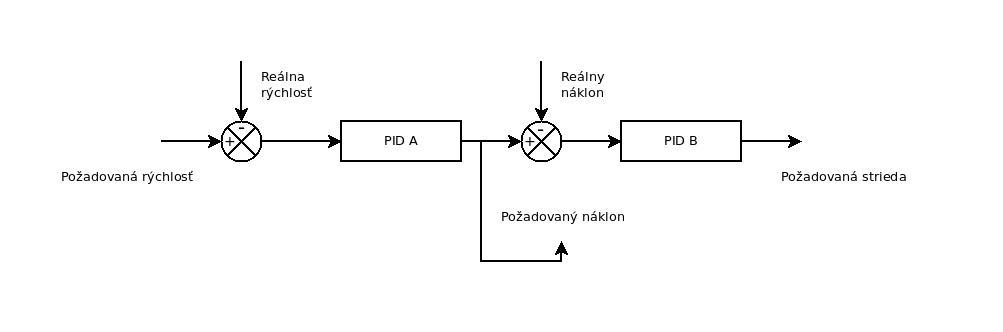
\includegraphics[width=10cm]{PID_robota}
\caption{Schematické zapojenie PID regulátorov}
\label{fig:RS}
\end{figure}

\underline{\textbf{PID A}}:
Vstupom do PID A je požadovaná rýchlosť robota, tá je odčítaná od reálnej rýchlosti nameranej pomocou enkodérov a spracovaná. Pri riadení robota môžeme špecifikovať požadovanú rýchlosť a na výstupe  PID A bude požadovaný uhol náklonu. Týmto spôsobom zabezpečíme ako dosiahnutie požadovanej rýchlosti tak aj to, že robot sa bude pohybovať konštantnou rýchlosťou. Výhodnou vlastnosťou PID A je, že požadovaný uhol náklonu nebude počas celej doby riadenia konštantný pre danú rýchlosť, ale bude dynamicky prispôsobovaný aktuálnym podmienkam. Ak by to tak nebolo robot by pri konštantnom uhle náklonu pokračoval v zrýchľovaní aby sa vyhol pádu až pokiaľ by motory dosiahli maximálnu rýchlosť a neboli schopné dosiahnuť požadované zrýchlenie na udržanie uhla náklonu. Po tomto bode by nasledoval pád.

\underline{\textbf{PID B}}:
Výstupom PID B je ako už bolo skôr spomenuté strieda signálu vstupujúceho do H-mostíka. V prípade nami použitého mostíka platí, priama úmera medzi striedou vstupného signálu a napätím do motorov. Nedá sa ale povedať, že by závislosť medzi striedou a výstupným napätím bola lineárna. V skutočnosti pre efektívne napätie na výstupe mostíka platí vzťah \eqref{eq:RMSSquare}, v ktorom $\delta$ je z intervalu $<0;1>$ a predstavuje striedu vstupného signálu. Závislosť výstupného napätia a striedy je zobrazená na \figurename~\ref{fig:strieda_napatie}. V našom prípade sa ale nejedná o závažný nedostatok, ktorý by výrazným spôsobom ovplyvňoval výsledky regulácie.

\begin{equation}
V_{EF} = V_{MAX}\sqrt{\delta}
\label{eq:RMSSquare}
\end{equation}

\begin{figure}[b]
\centering
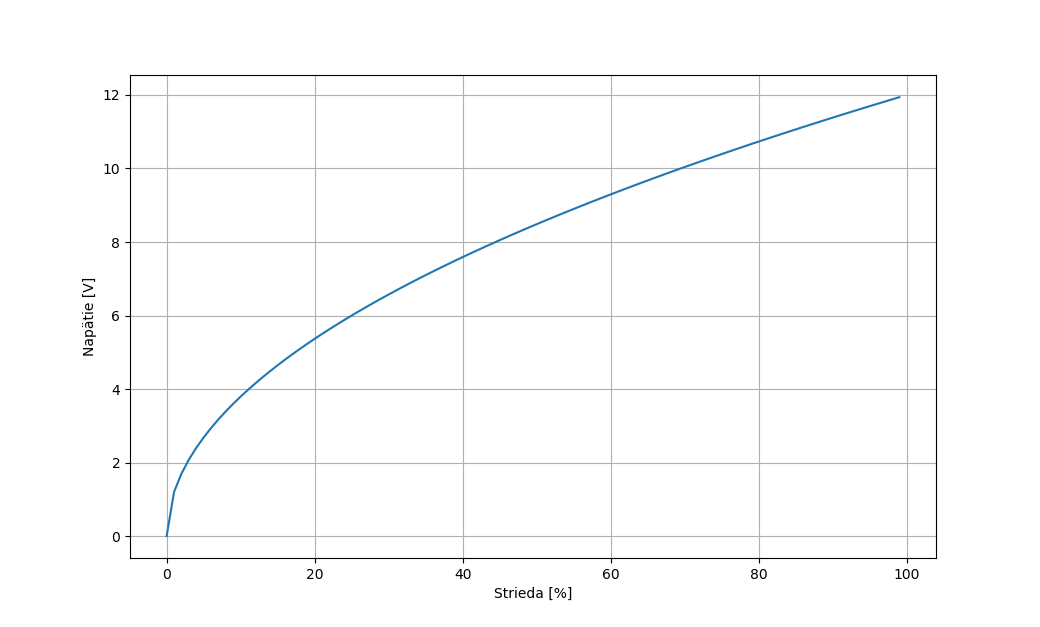
\includegraphics[width=10cm]{strieda_napatie}
\caption{Znázornenie závislosti medzi striedou a napätím}
\label{fig:strieda_napatie}
\end{figure}

Ladenie \ac{RS} prebiehalo po častiach. Ko prvý sme naladili PID B, pričom využitá bola Zieger-Nicholsova metóda, nasledovaná jemným, manuálnym doladením parametrov. Pri ladení bol na vstup privedený nulový vstupný signál, reprezentujúci požiadavku na nulový uhol náklonu. Výseldkom tohto ladenia bol robot schopný balancovať vo vzpriamenej polohe, ktorý odolal aj silnejším pokusom o jeho prevrhnutie. Ako nedostatkom sa ale javilo to, že robot nebol nijakým spôsobom penalizovaný za pohyb a tak trvalo aj niekoľko sekúnd kým sa po postrečení opäť dostal do ustáleného stavu (stav charakterizovaný minimálnou osciláciou okolo osi natočenia a minimálnou rýchlosťou pohybu).

Po naladení PID B, bol ladený PID A, pričom sme na vstup RS opäť priviedli nulovú hodnotu - teda požiadavku na nulovú rýchlosť. Keďže pri prevádzke bude práve tento stav s nulovou požiadavkou najčastejší pri ladení PID A sa kládol silný dôraz na správanie systému pri návrate do ustáleného stavu. PID A bol naladený obdobným spôsobom ako PID B. Výsledkom bol \ac{RS} schopný zabezpečiť minimálnu uhlovú výchylku robota pri minimálnej rýchlosti pohybu.

Keďže pri realizáciu PID bola použitá forma popísaná v \ref{eq:compPID} bole ešte potrevné určiť konštantu $T_f$ podľa vzťahu \ref{eq:TFconst}. Pri zisťovaní oscilačnej frekvencie robota pri pohybe sme na presné nameranie krátkych periód oscilácií použili kamerový záznam pohybu robota. Pri známej frekvencií snímkovania, ktorá bola v našom prípade 60 \ac{FPS}(frames per second), je spočítaním snímok a ich vynásobením periódou snímokovania možné presne odmerať aj krátke časové okamihy. Zavedenie konštanty $T_f$ zlepšilo vlastnosti \ac{RS} robota.

\section{Implementácia riadiaceho systému}
Implementácia \ac{RS} robota bola realizovaná v jazyku C++, pričom sme využili objektovo orientovaný spôsob programovania. V praxi to znamená, že jednotlivé funkčné celky robota sú reprezentované v dátových štruktúrach nazývaných objekty. Každý objekt predstavuje inštanciu triedy, v ktorej sú definované jeho vlastnosti a metódy - teda jeho štruktúra. Prostredníctvom týchto vlastností a metód objekt vykonáva vrámci funkčného celku určité funkcie. Výhodou tohto postupu je, že takto napísaný kód je znovupoužiteľný aj v iných projektoch a v prípade potreby jednoducho rozšíriteľný o dodatočnú funkcionalitu.

Príkladom triedy v nami použitom kóde je trieda \textit{PID}. V tejto triede sú definované metódy, ktoré by mal byť každý objekt triedy PID schopný poskytnúť. V našom prípade sa jedná o metódy pre nastavenie a úpravu parametrov P, I, D a metódu pre vypočítanie výstupe PIDu vzhľadom na určitý vstup. Vytvorenie tejto triedy nám umožní reprezentrovať PID A a PID B ako inštancie tejto triedy. 

Pri triede PID je treba poznamenať, že priame použitie \ref{eq:compPID} na vypočítanie výstupu by nebolo možné, kedže v nami predstavenej forme sa jedná o spojitý regulátor. Mikroprocesor je ale digitálne zariadenie, ktoré nie je schopné priamo realizovať spojitú funkciu, ani prijímať spojité dáta (ktoré by väčšina nami použitých senzorov ani nebola schopná poskytnúť). Je preto potrebné vyjadriť \ref{eq:compPID} aj vo spojitej forme. Výstup PID pre vzorku číslo $i$ je teda:

\begin{equation}
y_i = Pe_i + I\sum_{k=0}^{i}{e_k}\Delta t + D\Delta e_i 
\end{equation}
\begin{equation}
\Delta e_i = \dfrac{T_f\Delta e_{i-1} + (e_i - E_{i-1})}{\Delta t + T_f}
\end{equation}
pričom $e_i$ je rozdiel požadovaného uhla a skutočného uhla, pre vzorku $i$ a $\Delta t$ je čas medzi jednotlivými vzorkami.

\listingname~\ref{lst:PIDsample} predstavuje ukážku jednej nami implementovanej metódy triedy PID. Jej výstup predstavuje výstup daného PID regulátora.  


\begin{inlinecode}[label={lst:PIDsample},caption={Príklad jednej z metód triedy PID}]{c++}
float PID::giveOutput(float input, float target, float dt, float constrainI){
    float output  = 0;
    float Perror = target-input;
    error_integral += Perror;
    if(constrainI){
        error_integral = constrain(error_integral,-constrainI,constrainI);
    };
    error_derivative = (Tf*error_derivative + (Perror - old_error))/(dt + Tf);       //implements filtering constant Tf
    output = P*(Perror)+I*(error_integral)*dt+D*error_derivative;

    old_error = Perror;
    return output;
}
\end{inlinecode}

Celý nami vytvorený kód pracuje po úvodnej incializácií premenných a vytvorení objektov na princípe kontrolnej slučky, t.j. skupiny príkazov, ktoré sa periodicky opakujú. V našom prípade sme túto slučku navrhli tak aby prebehla raz za každých 10 ms. V tejto riadiacej slučke načítavame nové údaje zo senzorov, spracúvavame ich prostredníctvom \ac{RS} a na vstup H-mostíka privádzame výsledný signál \ac{PWM}. Celý proces je znázornený v diagrame \figurename~\ref{fig:simpleFlowchart}.

V \figurename~\ref{fig:simpleFlowchart} nie sú znázornené spracovania prerušení, v ktorých sa spracúvajú údaje z enkodérov, použitých na monitorovanie aktuálnej rýchlosti robota. Výstup zo samotných enkodérov prichádza do mikropočítača po štyroch dátových linkách (dve pre každý enkodér), vo forme impulzov vzájomne oneskorených o čas $t_e$. Výstup z dvoch kanálov enkodéra je zobrazený na \figurename~\ref{fig:enkoder} Na jedinú otáčku kolesa pripadá $N$ takto vzájomne posunutých impulzov. Spočítaním týchto impulzov za čas  $t_S$ vieme určiť uhlovú rýchlosť kolesa a z nej následne odvodiť celkovú rýchlosť pohybu robota. Smer pohybu určíme podľa poradia detekcie impulzov.

Vzorec pre výpočet pohybu robota je teda možné vyjadriť ako:
\begin{align*}
\phi_w &= \dfrac{2\pi}{N}k \qquad [rad] \\
\omega &= \dfrac{\phi_w}{t_S} \qquad [rad.s^{-1}]\\
v &= \omega r \qquad[m.s^{-1}]
\end{align*}
kde $k$ predstavuje počet detekovaných impulzov z jednej linky a $r$ polomer kolesa robota.

Následne je ešte potrebné zredukovať šum prítomný v takto nameraných dátach, v našom prípade pomocou komplementárneho filtra. Komplementárny filter bol taktiež použitý aj pri filtrovaní a fúzií dát nameraných z akcelerometra a gyroskopu.  

Podrobná schéma zobrazujúca celkovú činnosť \ac{RS} robota je na \figurename~\ref{fig:podrobna_schema}. Znázorňuje ako RS robota, tak aj spôsob spracovania dát na jeho vstupoch.

\begin{figure}[b]
\centering
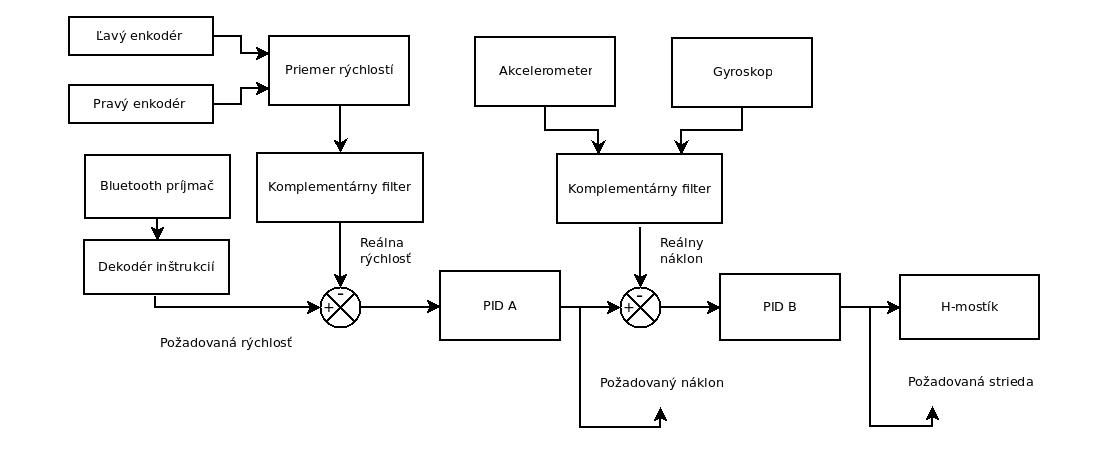
\includegraphics[width=15cm]{comp_RS_diagram}
\caption{Podrobná schéma RS robota}
\label{fig:podrobna_schema}
\end{figure}


